\documentclass{beamer}
\usetheme[block=fill, subsectionpage=progressbar]{metropolis}

\usepackage{amsmath}
\usepackage[style=numeric]{biblatex}
\usepackage{url}

\addbibresource{references.bib}

\title{Modelling Baseball Exit Velocities with Extreme Value Theory}
\subtitle{MATH 589 Final Project}
\author{Jules Lanari-Collard}
\institute{McGill University}
\date{November 29, 2024}

\begin{document}
\frame{\titlepage}
\section{Introduction}

\begin{frame}{Why?}
\begin{itemize}
    \item Average MLB franchise is worth \$2.4 billion \cite{forbesValuations}.
    \item 2nd most popular sport in US \cite{gallupPoll}.
    \item Median projected payroll for 2025 is \$144 M - some teams projected for over \$270 M \cite{fgRosterResource}.
    \item Shohei Ohtani signed for \$700 M over 10 years (2024-2033).
    \item Franchises employ dedicated analytics teams to inform decisions and evaluate players.
\end{itemize}
\end{frame}

\begin{frame}[allowframebreaks]{Why Exit Velocity Matters}
    \begin{figure}
        \centering
        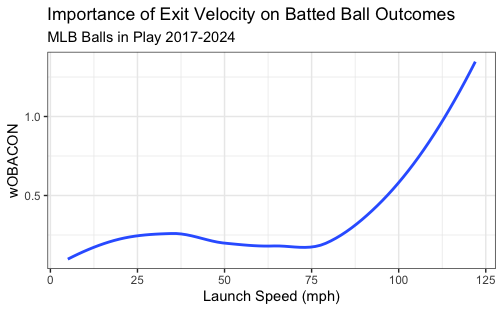
\includegraphics[width=\linewidth]{plots/ev_woba.png}
        \label{fig:ev_woba}
    \end{figure}
    \begin{figure}
        \centering
        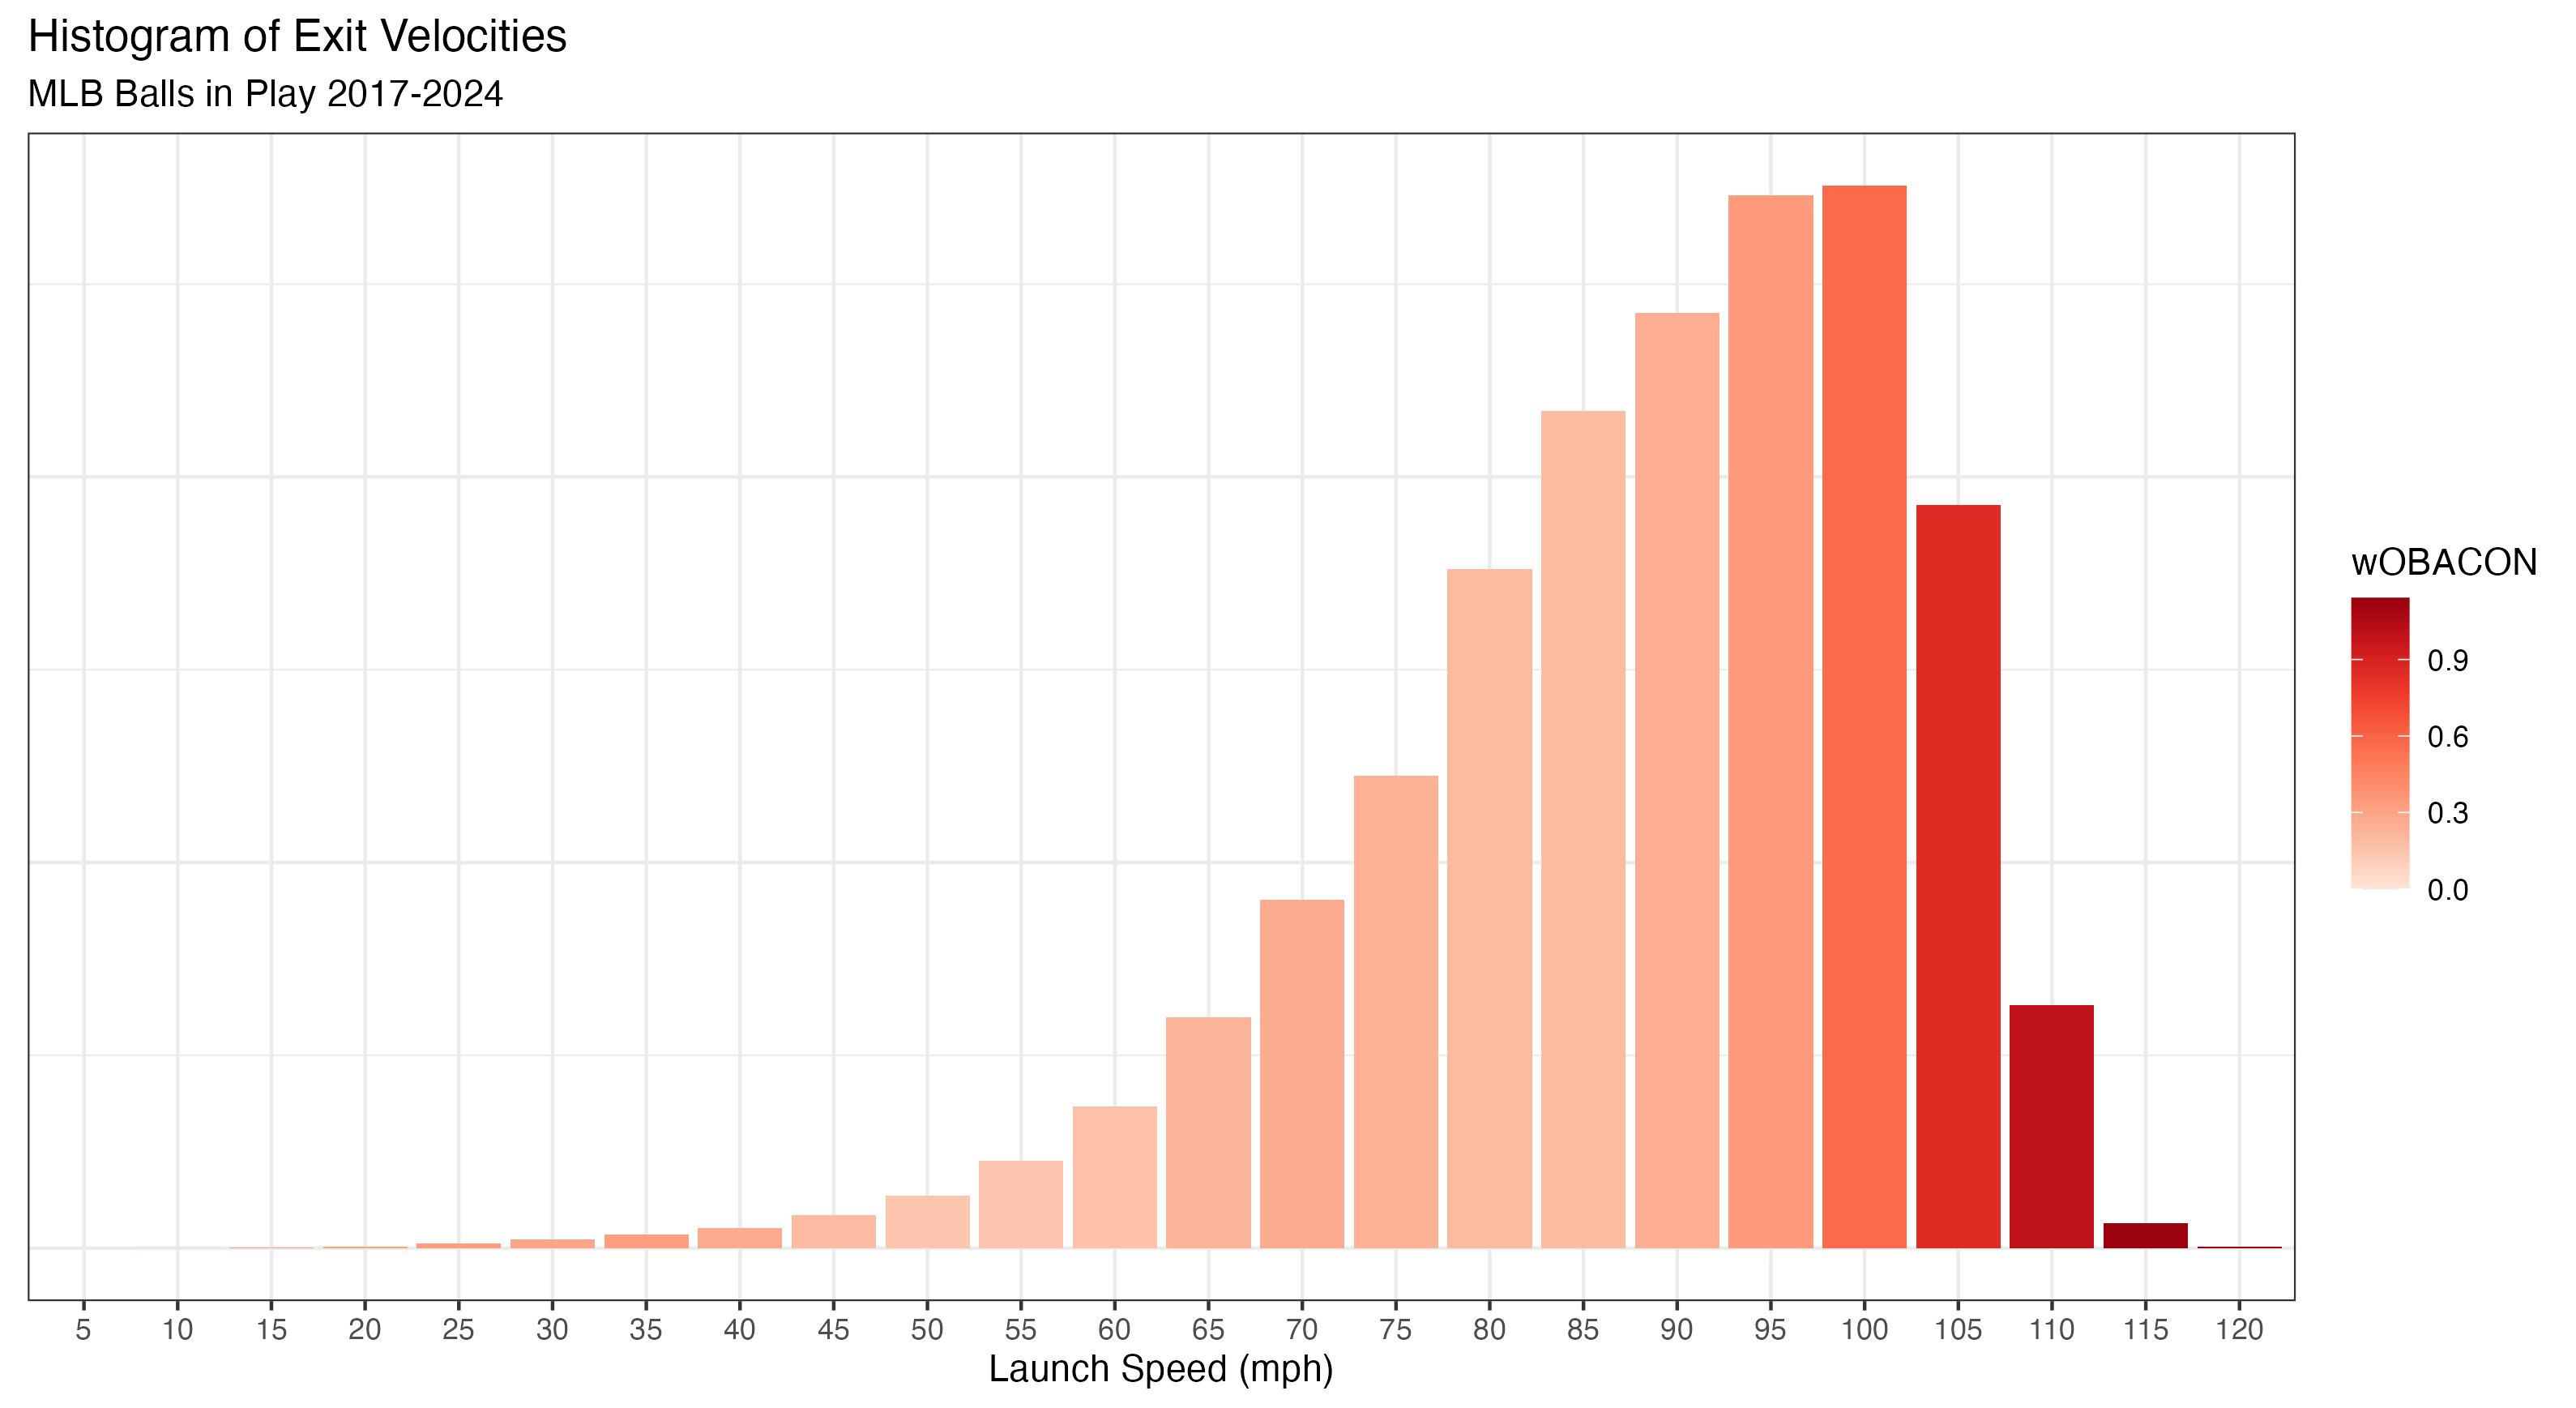
\includegraphics[width=\linewidth]{plots/evHistogram.png}
        \label{fig:evHistogram}
    \end{figure}
\end{frame}

\begin{frame}{Player Distributions}
    Differing player types \& styles lead to different player-level EV distributions:
    \begin{figure}
        \centering
        \includegraphics[width=0.5\linewidth]{}
        \caption{Caption}
        \label{fig:enter-label}
    \end{figure}
\end{frame}

\begin{frame}{Existing Exit Velocity Metrics}
\begin{itemize}
    \item Average EV
    \item Best Speed \cite{tangoBestSpeed}
    \begin{itemize}
        \item Average of top 50\% hardest-hit balls
    \end{itemize}
    \item EV Percentiles \cite{clemensEV}
    \begin{itemize}
        \item EV80, EV90 \& EV95
    \end{itemize}
    \item Maximum EV
    \item Hard-Hit \%
    \begin{itemize}
        \item \% of balls hit $>$95mph
    \end{itemize}
\end{itemize}
\end{frame}

\section{A New Approach}


\begin{frame}[allowframebreaks]
    \printbibliography
\end{frame}
\end{document}